% LaTeX source for ``การเรียนรู้ของเครื่องสำหรับเคมีควอนตัม (Machine Learning for Quantum Chemistry)''
% Copyright (c) 2022 รังสิมันต์ เกษแก้ว (Rangsiman Ketkaew).

% License: Creative Commons Attribution-NonCommercial-NoDerivatives 4.0 International (CC BY-NC-ND 4.0)
% https://creativecommons.org/licenses/by-nc-nd/4.0/

\chapter{คุณสมบัติเชิงอิเล็กทรอนิกส์ของโมเลกุล}
\label{ch:el_prop}

เนื้อหาในบทนี้จะเกี่ยวกับคุณสมบัติเชิงอิเล็กทรอนิกส์ (Electronic Properties) ของโมเลกุล ซึ่งเป็นวัตถุประสงค์ของการใช้ ML เข้ามาศึกษาเคมีควอนตัม
โมเลกุลเป็นหน่วยพื้นฐานของสิ่งต่าง ๆ รอบตัวเรา ซึ่งโมเลกุลก็คือเป็นกลุ่มของอะตอมหลาย ๆ อะตอมมารวมกัน และในอะตอมนั้นเราสนใจอิเล็กตรอนเป็นพิเศษ
ในวิชาควอนตัมนั้นเราจะอธิบายพฤติกรรมของโมเลกุลโดยมุ่งเน้นไปที่อิเล็กตรอนซึ่งสามารถที่จะอธิบายได้ด้วยฟังก์ชันทางคณิตศาสตร์ที่เรียกว่าฟังก์ชันคลื่น 
(Wavefunction) โดยหน้าตาของ Wavefunction นั้นจริง ๆ แล้วไม่มีการนิยามแบบตายตัว โดยหนึ่งในสมการที่โด่งดังที่สุดสมการหนึ่งของวงการ%
วิทยาศาสตร์นั่นคือสมการชโรดิงเงอร์ (Schrödinger Equation) โดยถูกนำมาใช้ในการศึกษาระบบทางกลศาสตร์ควอนตัม ซึ่งการแก้สมการชโรดิงเงอร์%
ได้นั้นจะทำให้ได้มาซึ่ง Wavefunction 

สมการชโรดิงเงอร์สามารถแบ่งออกได้เป็นสองแบบ คือ แบบที่ไม่ขึ้นกับเวลาและแบบที่ขึ้นกับเวลา ดังนี้\cite{szabo1996,cramer2004,jensen2017}

\noindent Time-dependent Schrödinger Equation

\begin{equation}
    i \hbar \frac{d}{d t} \ket{\Psi(t)} = \hat{H} \ket{\Psi(t)}
\end{equation}

\noindent Time-independent Schrödinger Equation

\begin{equation}
    \hat{H}\ket{\Psi} = E \ket{\Psi}
\end{equation}

โดย Wavefunction ($\Psi(t)$) ที่เป็น Eigenfunction นั้นจะบรรจุข้อมูลเชิงอิเล็กทรอนิกส์ทุกอย่างเกี่ยวกับระบบของเราเอาไว้ ซึ่งในที่นี้ก็คือโมเลกุล
โดยสมการข้างต้นเป็นการคำนวณหาพลังงานของระบบโดยใช้ Hamiltonian Operator ($\hat{H}$) ซึ่งเป็น Operator ที่สอดคล้องกับพลังงาน
ซึ่งจริง ๆ แล้ว Eigenvalue ของสมการข้างต้นจะเป็นคุณสมบัติของโมเลกุลอะไรก็ได้ ตราบใดที่เราใช้ Operator ที่สอดคล้องกับคุณสมบัตินั้น ๆ 

หนึ่งในเป้าหมายสำคัญของกลศาสตร์ควอนตัมเชิงโมเลกุลก็คือการแก้สมการ Time-independent Schrödinger Equation และคำนวณหาโครงสร้าง%
เชิงอิเล็กทรอนิกส์ (Electronic Structures) ของอะตอมและโมเลกุล โดยหัวข้อแรกของบทนี้ที่เราจะมาดูกันแบบละเอียดก็คือการใช้เทคนิคเชิงคำนวณ%
และอาศัยการประมาณค่าในการแก้สมการดังกล่าว โดยทั่วไปนั้นจะมีวิธีการหลัก ๆ 2 วิธีที่สามารถช่วยให้เราหาคำตอบของสมการชโรดิงเงอร์ ได้นั่นคือ 
\textbf{\textit{ab initio} method} ซึ่งเป็นวิธีที่ความถูกแม่นยำของผลลัพธ์ที่ได้จากการแก้สมการนั้นจะขึ้นอยู่กับโมเดลที่เรานำมาใช้ในการ%
อธิบาย Wavefunction ของโมเลกุล และเป็นที่ทราบกันดีว่าสำหรับโมเลกุลที่มีขนาดใหญ่นั้น วิธีการ \textit{ab initio} นี้จะมีความสิ้นเปลืองสูงมาก 
ดังนั้นจึงเป็นที่มาของวิธีการที่สอง นั่นคือ \textbf{Semiempirical method} ซึ่งจะใช้เทคนิคการมอง Hamiltonian ในรูปแบบที่ง่ายกว่า 
และอาศัยค่า Parameter ที่ได้จากการทดลองเพื่อเพิ่มความแม่นยำ อย่างไรก็ตาม วิธี Density Functional Theory (DFT) ก็ถูกพัฒนาขึ้นมา%
เพื่อแก้ปัญหาที่เราจะต้องมาแก้หรือประมาณค่า Wavefunction ตรง ๆ จึงทำให้ความสิ้นเปลืองของการคำนวณนั้นต่ำมากเมื่อเทียบกับสองวิธีข้างต้นทีได้กล่าวไป

%--------------------------
\section{การแก้สมการฟังก์ชันคลื่นเพื่อคำนวณพลังงาน}
%--------------------------

%--------------------------
\subsection{วิธี Self-Consistent Field}
%--------------------------

ในหัวข้อนี้เราจะมาพูดถึงการแก้สมการชโรดิงเงอร์โดยใช้วิธีที่ชื่อว่า Self-Consistent Field (SCF) ซึ่งเป็นการประมาณค่า Hamiltonian แบบวนซ้ำ
เริ่มต้นเราจะต้องมาดูกันก่อนว่าการมอง Wavefunction ของระบบหลายอิเล็กตรอนสำหรับวิธี SCF นั้นจะมีการตัดสิ่งที่ซับซ้อนออกไปนั่นก็คือ
Electron-Electron Repulsion หรืออันตรกิริยาระหว่างอิเล็กตรอน โดย Wavefunction สามารถถูกอธิบายได้ด้วยสมการต่อไปนี้\cite{cramer2004}

\begin{equation}
    H^{\circ} \Psi^{\circ} = E^{\circ} \Psi^{\circ}
\end{equation}

โดยกำหนดให้ $H^{\circ} = \sum^{N}_{i=1} h_{i}$ เมื่อ $h$ คือ Hamiltonian สำหรับหนึ่งอิเล็กตรอน (อิเล็กตรอนตัวที่ $i$) 
ในระบบที่มีอิเล็กตรอน $N$ ตัว นั่นคือสมการสำหรับระบบที่มีอิเล็กตรอน $N$ ตัวนั้น จะสามารถถูกแยกออกมาได้เป็นสมการของระบบหนึ่งอิเล็กตรอนได้ 
$N$ สมการ และ Wavefunction ของอิเล็กตรอนหนึ่งตัวนั้นจริง ๆ แล้วก็คือออร์บิทัล (Orbital) เราจึงสามารถเขียนสมการของอิเล็กตรอนหนึ่งตัวได้เป็น

\begin{equation}
    h_{i} \Psi^{\circ}(i) = E^{\circ}_{m} \Psi^{\circ}(i)
\end{equation}

\noindent โดยที่ $E^{\circ}_{m}$ คือพลังงานของอิเล็กตรอนหนึ่งตัวใน Molecular Orbital (MO) ซึ่งเขียนแทนด้วย $m$ นั่นเอง สำหรับระบบที่%
อิเล็กตรอนไม่ขึ้นต่อกันและกัน

ด้วยเหตุนี้ Wavefunction รวมของระบบ ($\Psi^{\circ}$) จึงสามารถเขียนให้อยู่ในรูปของ Wavefunction ของอิเล็กตรอนหนึ่งตัวได้ดังนี้

\begin{equation}
    \Psi^{\circ} = \psi^{\circ}_{a}(1) \psi^{\circ}_{b}(1) \dots \psi^{\circ}_{z}(N)
\end{equation}

\noindent ซึ่ง Wavefunction ด้านบนนี้จะขึ้นอยู่กับพิกัดของอิเล็กตรอนทุกตัวและขึ้นกับตำแหน่งของนิวเคลียสหรืออะตอมด้วย%
\footnote{ตอนนี้เราจะยังไม่พิจารณาสปินของอิเล็กตรอนที่จะต้องสอดคล้องและไม่ขัดกับหลักกีดกันของเพาลีหรือ Pauli Exclusion 
ซึ่งจะมีการรวม Spinorbital สำหรับ Molecular Orbital $m$ ($\varphi_{m}$) เข้าไปด้วย}

สำหรับกระบวนการหรือขั้นตอนที่เราจะนำมาใช้ในการแก้สมการของระบบอิเล็กตรอนหลายตัวนั้น เราจะพิจารณาสมการรูทฮาน (Roothaan Equation) 
เป็นหลัก ซึ่งเป็นวิธีหนึ่งในการแก้สมการ Hartree-Fock (HF) ซึ่งมีการกำหนดตัวดำเนินการใหม่ขึ้นมาใช้แทน Hamiltonian นั่นก็คือ Fock Operator 
โดยที่ Fock Operator ถูกนิยามในเทอมของ Coulomb Operator และ Exchange Operator ขึ้นมา นั่นก็คือ Fock Operator 
ซึ่งเขียนสมการสำหรับอิเล็กตรอน 1 ตัวได้เป็น

\begin{equation}
    \label{eq:fock}
    f_{1} \psi_{m}(1) = \varepsilon_{n} \psi_{m}(1)
\end{equation}

%--------------------------
\subsection{สมการ Roothaan}
%--------------------------

สำหรับการแก้สมการ HF ตรง ๆ โดยใช้ SCF นั้นสามารถทำได้ตรง ๆ ด้วยวิธีการเชิงตัวเลข (Numerical Method) แต่ว่าผลเฉลยที่ได้มานั้นมีความ%
ซับซ้อนมาก โดยในเวลาต่อมานักฟิสิกส์และนักเคมีชาวดัตช์ที่ชื่อว่า Clemens C.J. Roothaan จึงได้เสนอวิธีการใหม่สำหรับการอธิบาย MO โดยเรียก%
วิธีนั้นว่า Linear Combination of Atomic Orbitals (LCAO) เรามาดูกันเลยว่าวิธีการนี้มีรายละเอียดอย่างไร\cite{atkins2010}

เริ่มต้นเราจะนิยามฟังก์ชันพื้นฐาน (Basis Function) สำหรับระบบที่มีอิเล็กตรอน $N$ ตัวขึ้นมาก่อน ซึ่งเขียนแทนด้วย $\chi_{o}$
ซึ่งไอเดียตอนนี้ก็คือเราจะมองว่า Basis Function แบบที่ง่ายที่สุดที่เราสามารถนำมาใช้ได้นั่นก็คือ Atomic Orbital (O) ซึ่งสามารถที่จะเขียน 
Spatial Wavefunction (ฟังก์ชันคลื่นที่ขึ้นกับตำแหน่ง ของ AO) ให้อยู่ในผลรวมเชิงเส้นของการคูณระหว่างสัมประสิทธิ์เชิงเส้นที่เรายังไม่ทราบค่า 
(Unknown Coefficients, $c_{om}$) กับ $\chi_{o}$ ดังนี้

\begin{equation}
    \label{eq:lcao}
    \psi_{m} = \sum^{N_{o}}_{o=1} c_{om} \chi_{o} 
\end{equation}

\noindent เมื่อเราแทนสมการ \ref{eq:lcao} เข้าไปในสมการ \ref{eq:fock} เราจะได้

\begin{equation}
    \label{eq:lcao_in_fock}
    f_{1} \sum^{N_{o}}_{o=1} \chi_{o}(1) = \varepsilon \sum^{N_{o}}_{o=1} c_{om} \chi_{o}(1)
\end{equation}

\noindent แล้วทำการคูณสมการ \ref{eq:lcao_in_fock} ทั้งสองข้างด้วย $\chi^{*}_{o}(1)$ และทำการอินทิเกรตทั่วทั้ง Space ซึ่งจะทำให้เราได้%
ความสัมพันธ์ต่อไปนี้

\begin{equation}
    \label{eq:lcao_in_fock_int}
    \sum^{N_{o}}_{o=1} c_{om} \int \chi^{*}_{o}(1) f_{1} \chi_{o}(1) d\tau_{1} =
    \varepsilon_{m} \sum^{N_{o}}_{o=1} c_{om} \int \chi^{*}_{o}(1) \chi_{o}(1) d\tau_{1}
\end{equation}

\noindent จากสมการข้างต้นเราจะพบว่าจะมีผลคูณของ Basis Function ทั้งสองฝั่ง โดยทางฝั่งซ้ายนั้นเราสามารถนิยาม Fock Matrix (F) ได้

\begin{equation}
    \label{eq:matrix_fock}
    F_{o'o} = \int \chi^{*}_{o'}(1) f_{1} \chi_{o}(1) d\tau_{1}
\end{equation}

\noindent และทางฝั่งขวา เรานิยามสิ่งที่เรียกว่า Overlap Matrix (S) ซึ่งเป็น Matrix ที่อธิบายถึงการซ้อนทับกันระหว่างสถานะ 2 สถานะ

\begin{equation}
    \label{eq:matrix_overlap}
    S_{o'o} = \int \chi^{*}_{o'}(1) \chi_{o}(1) d\tau_{1}
\end{equation}

\noindent ซึ่งเราสามารถเขียนสมการ \ref{eq:lcao_in_fock_int} ให้อยู่ในรูปของสมการที่เรียกว่า Roothaan Equation ได้กระชับ ๆ ดังนี้

\begin{equation}
    \label{eq:roothaan}
    F c = \varepsilon S c
\end{equation}

\noindent โดยที่ $c$ คือเมทริกซ์ขนาด $N_{o} \times N_{o}$ ซึ่งประกอบไปด้วยสมาชิกของ Coefficient $c_{om}$ และ $\varepsilon$ 
คือเมทริกซ์ที่มีขนาด $N_{o} \times N_{o}$ เช่นเดียวกันซึ่งเป็นเมทริกซ์แบบ Diagonal Matrix (สมาชิกที่ไม่ใช่แนวทแยงมีค่าเป็น 0 ทั้งหมด) 
ซึ่งก็คือพลังงานของ Orbital นั่นเอง ซึ่งตรงจุดนี้เราต้องไม่ลืมว่า Fock Operator ($f_{1}$) นั้นถูกกำหนดให้อยู่ในรูปของ Integral บน MO 
และขึ้นอยู่กับค่าของ Coefficient $c_{om}$ ด้วย

สำหรับการแก้สมการ \ref{eq:roothaan} นั้นสามารถทำได้ผ่าน Determinant ดังนี้

\begin{equation}
    \label{eq:scf_secular}
    det|F - \varepsilon S| = 0
\end{equation}

\noindent ซึ่งสมการด้านบนไม่สามารถแก้ได้แบบตรงไปตรงมาเพราะว่าสมาชิกของเมทริกซ์ $F_{o'o}$ นั้นเกี่ยวเนื่องโดยตรงกับ Integral ของ 
Coulomb Operator และ Exchange Operators ซึ่งขึ้นอยู่กับ Spatial Wavefunction นั่นจึงทำให้เป็นปัญหาแบบงูกินหาง ดังนั้นเราจึงต้อง%
ใช้กระบวนการวนซ้ำ (Iteration) ในการแก้ปัญหาจนกว่าคำตอบหรือผลลัพธ์ที่เราต้องการจากสมการ (พลังงาน) จะลู่เข้านั่นเอง

%--------------------------
\subsection{การแก้สมการ Roothaan ด้วย Self-Consistent Field}
%--------------------------

\begin{figure}[H]
    \centering
    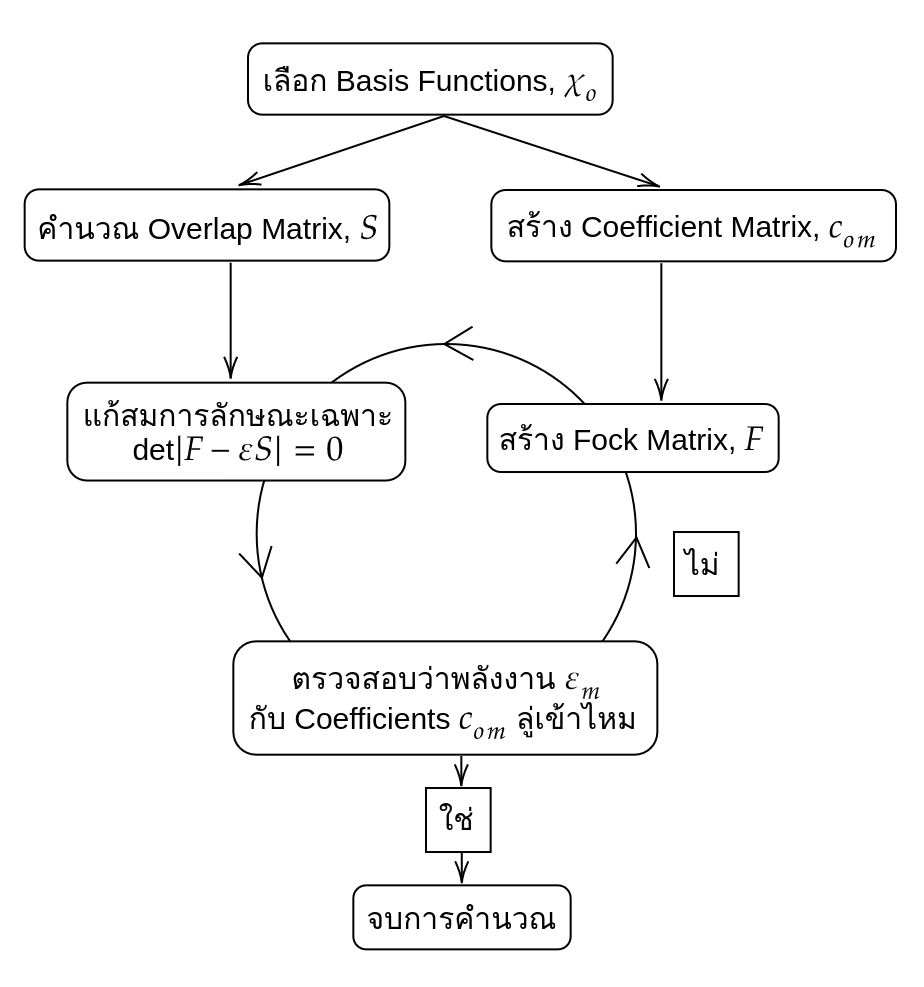
\includegraphics[width=0.8\linewidth]{fig/scf.png}
    \caption{แผนผังขั้นตอนของ SCF ในการประมาณค่าหาพลังงานของออร์บิทัล}
    \label{fig:scf}
\end{figure}

ภาพที่ \ref{fig:scf} แสดงแผนผงอัลกอริทึมของวิธี SCF โดยเริ่มจากการเลือก Atomic Basis Function ซึ่งถือว่าเป็นองค์ประกอบหลักของ%
การนำไปสร้าง (Formulate) $S$ โดยใช้สมการ \ref{eq:matrix_overlap} กับ $c_{om}$ ซึ่งเราจะใช้วิธีการสร้างค่าเริ่มต้นด้วยวิธี Guess 
ซึ่งมีด้วยกันหลายวิธี เช่น

\begin{enumerate}
    \item \textbf{H{\"u}ckel guess} : ใช้ H{\"u}ckel Orbital\cite{jensen2017}
    \item \textbf{Superposition of Atomic Densities (SAD)} : ใช้ผลรวมของ Atomic Density ในการสร้าง Density Matrix
    \item \textbf{Generalized Wolfsberg-Helmholtz (GWH)} : เป็นวิธีการที่อาศัย H{\"u}ckel Theory โดยการใช้ Overlap 
    Matrix และ Core Hamiltonian\cite{wolfsberg1952}
    \item \textbf{CORE} : ทำการทำ Core Hamiltonian ให้เกิดเมทริกซ์รูปทแยง (Diagonalization)
    \item \textbf{Harris} : ใช้ Harris Functional ซึ่งเป็น Non-self-consistent Approximation สำหรับ Kohn-Sham 
    Orbital\cite{harris1985}
\end{enumerate}

ซึ่งโปรแกรมเคมีเชิงคำนวณต่างก็มีการเลือกใช้ Guess Method สำหรับการเดา Coefficient หรือ Wavefunction เริ่มต้นในการแก้ SCF แตกต่างกันไป
โปรแกรม Gaussian ใช้วิธี Harris สำหรับการคำนวณ HF และ DFT และใช้ H{\"u}ckel หรือ CORE สำหรับ Semiempirical Methods, 
โปรแกรม Q-Chem และ Psi4 ใช้วิธี SAD กับ GWH เป็นวิธีเริ่มต้นโดยอัตโนมัติ เป็นต้น

หลังจากสร้าง Coefficient Matrix ขั้นตอนต่อไปคือการสร้าง Fock Matrix $F$ โดยใช้สมการ \ref{eq:matrix_fock} 
หลังจากนั้นเราจะทำการแก้สมการลักษณะเฉพาะ (Secular Equation) สมการที่ \ref{eq:scf_secular} เพื่อหา Energy Matrix 
แล้วก็ทำการวนซ้ำขั้นตอนการสร้าง $S$ กับ $F$ ไปปรับหาค่าพลังงานไปเรื่อย ๆ จนกว่าค่าความคลาดเคลื่อนหรือ Error จะมีค่าน้อยกว่าค่าที่กำหนดไว้ 
(Threshold) แล้วจึงสิ้นสุดกระบวนการ SCF เมื่อค่าพลังงานนั้นลู่เข้า

%--------------------------
\subsection{การคำนวณอนุพันธ์ของพลังงานและเมทริกซ์เฮสเซียน}
\idxen{Energy Derivative}
%--------------------------

หลังจากที่เราสามารถหาพลังงานเชิงอิเล็กทรอนิกส์ (Electronic Energy) ได้แล้ว ลำดับถัดไปที่เราสามารถคำนวณได้ก็คือคุณสมบัติต่าง ๆ ของโมเลกุล
สิ่งแรกที่เราทำได้และถือว่าสำคัญมาก ๆ ในงานวิจัยทางด้านเคมีควอนตัมก็คือการหาโครงสร้างที่เหมาะสมหรือเสถียรที่สุดของโมเลกุลโดยใช้หลักเกณฑ์%
พลังงานรวมที่ต่ำที่สุด ซึ่งการที่เราทราบโครงสร้างที่เหมาะสมที่สุดนั้นมีประโยชน์อย่างมากเพราะเราสามารถนำผลการคำนวณไปเทียบกับผลจากการทดลอง%
ด้วยเทคนิค X-ray Crystallography, Electron Diffractiom, หรือ Microwave Spectroscopy เป็นต้น โดยการหาโครงสร้างที่สภาวะ%
เหมาะสมหรือสมดุล (Equilibrium Structure) นั้นสามารถทำได้โดยหาอนุพันธ์ของพลังงานศักย์ของโมเลกุลเทียบกับพิกัดนิวเคลียร์ ซึ่งวิธีการที่%
เราสามารถนำมาหาอนุพันธ์เพื่อให้ได้ผลลัพเชิงวิเคราะห์ (Analytical Method) เรียกว่า Gradient Method ซึ่งเร็วและให้ผลลัพธ์ที่แม่นยำกว่า%
ระเบียบวิธีเชิงตัวเลข (Numerical Method)

สำหรับอนุพันธ์ของพลังงานนั้นเราจะเริ่มต้นพิจารณากรณีที่ง่าย ๆ นั่นก็คือโมเลกุลที่มีอะตอมสองอะตอม ซึ่งพลังงานศักย์ของโมเลกุลซึ่งเขียนแทนด้วย $E$ 
นี้จะมีเทอมที่เป็นแรงผลักระหว่างนิวเคลียสด้วยซึ่งจะขึ้นกับระยะห่างระหว่างนิวเคลียส (Internuclear Distance, $R$) สำหรับโครงสร้างที่อยู่ในสมดุลนั้น 
แรง (Force) ที่กระทำต่อนิวเคลียสโดยอิเล็กตรอนนั้นจะเท่ากับศูนย์ ซึ่งแรงดังกล่าวเป็นแรงย่อยมีนิยามคืออนุพันธ์อันดับที่หนึ่งของพลังงานศักย์เทียบ%
กับพิกัดของนิวเคลียสที่ $i$

\begin{align}
    f_{i} &= - \pdv{E}{q_{i}} \\
    &= 0
\end{align}

โดยการคำนวณหาอนุพันธ์ข้างต้นด้วยวิธีการวิเคราะห์หรือ Analytical Method นั้นเราจะต้องทำการคำนวณหาอนุพันธ์ของอินทิกรัลของอิเล็กตรอน%
หนึ่งตัวและอิเล็กตรอนสองตัว (One-electron กับ Two-electron Integrals) เทียบกับพิกัดนิวเคลียร์ นั่นคือเราจะต้องทำการหาอนุพันธ์ของ 
Basis Function นั่นเอง\footnote{Basis Function ก็คือ Basis ที่เกิดขึ้นมาจาก Atomic Orbtials ที่ถูก centered หรือมีตำแหน่ง%
อยู่ที่จุดอ้างอิงของนิวเคลียสของอะตอมในโมเลกุล} ซึ่งเราสามารถทำได้ผ่านการใช้กฎลูกโซ่ (Chain Rule) โดยทำการหาอนุพันธ์ของพลังงานศักย์%
เทียบกับ Expansion Coefficient

ลำดับถัดมาคือการหาเมทริกซ์เฮสเซียน (Hessian Matrix) ซึ่งสามารถทำได้โดยการหาอนุพันธ์ย่อยอันดับที่สองของพลังงานศักย์เทียบกับนิวเคลียส%
ของอะตอมตัวที่ $i$ และ $j$ ($\pdv{E}{q_{i}}{q_{j}}$) ซึ่งช่วยให้เราสามารถระบุได้ว่าค่าพลังงานที่คำนวณออกมาได้นั้นสอดคล้องกับ%
จุดต่ำสุดหรือสูงสุดบนพื้นผิวพลังงานศักย์ (Potential Energy Surface) โดยจะสอดคล้องกับอนุพันธ์อันดับที่สองที่ได้ค่าออกมาเป็นบวก 
(สำหรับ Minimum Point) และลบ (สำหรับ Maximum Point) ตามลำดับ

%--------------------------
\section{ความหนาแน่นเชิงประจุและเมทริกซ์ความหนาแน่น}
%--------------------------

ความหนาแน่นเชิงประจุ (Charge Density) เป็นปริมาณที่บ่งบอกถึงประจุของอะตอมที่อยู่ในโมเลกุล ถ้าหากเราทำการอินทิเกรต Charge Density 
ทั่วทั้งปริมาตรเราจะได้ผลลัพธ์เป็นจำนวนของอิเล็กตรอนในระบบของเรา (โมเลกุล) ดังนี้\cite{szabo1996}

\begin{equation}
    N = \int \rho (\mathbf{r}) dV
\end{equation}

โดยนิยามของ Charge Density จะเป็นผลรวมของโอกาสที่เราจะพบอิเล็กตรอนที่อยู่ภายใน Molecular Orbitals ของทั้งระบบ ดังนี้
\idxen{Charge Density}

\begin{equation}
    \rho (\mathbf{r}) = 2 \sum^{N/2}_{i=1} \int |\varphi_{i}(\mathbf{r})|^{2}
\end{equation}

\noindent โดยเลข 2 ด้านหน้าเครื่องหมาย Summation ก็คือ Occupation Number สำหรับกรณีที่ Molecular Orbital ($i$) 
นั้นมีอิเล็กตรอนทั้งแบบ Spin Up และ Spin Down และ $\varphi_{i}(\mathbf{r})$ คือ Wavefunction ซึ่งเราสามารถเขียน Wavefunction 
ให้อยู่ในรูปผลรวมเชิงเส้นของ Basis Function ($\phi_{i}$) ซึ่ง Basis Function นี้จะเป็นฟังก์ชันอะไรก็ได้ที่สามารถอธิบายการมีอยู่ของ 
Molecular Orbitals โดยในกรณีแบบที่ง่ายที่สุดคือเราจะมองว่า Molecular Orbitals นั้นเกิดขึ้นมาจากการรวมกันของ Atomic Orbitals 
ดังนั้นเราจะกำหนดให้ Atomic Orbitals เป็น Basis Function\footnote{Basis Function ในที่นี้คือ Atomic Orbitals ที่ถูกกำหนดให้%
มีจุดศูนย์กลางอยู่ที่อะตอมนั้น ๆ} ดังนั้นผลรวมเชิงเส้นดังกล่าวจึงมีเรียกว่า Linear Combination of Atomic Orbitals หรือ LCAO 
ตามสมการดังต่อไปนี้

\begin{equation}
    \rho (\mathbf{r}) = 2 \sum_{i} \big( \sum_{\mu} c_{\mu i} \phi_{\mu}^{*} \big) 
    \big( \sum_{\nu} c^{*}_{\nu i}  \phi_{\nu} \big)
\end{equation}

\noindent โดยที่ $c$ คือสัมประสิทธิ์ของ Linear Combination ของ Atomic Orbitals (LCAO) ลำดับต่อมาคือเมื่อเราจัดรูปให้มีเทอมที่%
เป็นผลคูณของ Basis Function ($\phi_{\mu}^{*} \phi_{\nu}$) เราจะกำหนดให้เทอมนี้เป็นสิ่งที่เรียกว่า Overlap Matrix ($S_{\mu\nu}$) 
โดยจะได้สมการที่จัดรูปแล้ว ดังนี้

\begin{equation}
    \rho (\mathbf{r}) = 2 \sum_{i}\sum_{\mu\nu} c_{\mu i} c^{*}_{\nu i} S_{\mu\nu}
\end{equation}

หลังจากนั้นเราจะพบว่าจะมีเทอมที่เป็นผลคูณระหว่าง $c$ ซึ่งเราจะกำหนดให้ผลคูณแบบนี้เรียกว่า Density Matrix 
($P_{\mu\nu} = c_{\mu i} c^{*}_{\nu i}$) ซึ่งเราจะได้สมการดังต่อไปนี้
\idxen{Density Matrix}

\begin{equation}     
    \rho (\mathbf{r}) = 2 \sum_{i} \sum_{\mu\nu} P_{\mu\nu}S_{\mu\nu}
\end{equation}

%--------------------------
\section{พลังงานของ Frontier Orbitals}
%--------------------------

\idxen{Frontier Orbitals}

\idxen{Ground State}

%--------------------------
\subsection{พลังงานของ HOMO และ LUMO}
\idxth{พลังงานของ HOMO และ LUMO}
%--------------------------

\idxen{Frontier Orbitals!HOMO}

\idxen{Frontier Orbitals!LUMO}

%--------------------------
\subsection{ผลต่างของพลังงานของ HOMO และ LUMO}
%--------------------------

\idxen{Energy Gap}

%--------------------------
\section{ไดโพลโมเมนต์}
%--------------------------

ไดโพลโมเมนต์ (Dipole Moment)

\idxen{Dipole Moment}

%--------------------------
\section{สภาพการเกิดขั้ว}
%--------------------------

สภาพการเกิดขั้ว (Polarizability)
\idxen{Polarizability}

%--------------------------
\section{เทคนิคสเปกโทรสโกปีแบบสั่น}
\idxen{Spectroscopy}
\idxen{Spectroscopy!Vibrational Spectroscopy}
%--------------------------

สเปกโทรสโคปี (Spectroscopy) เป็นการศึกษาอันตรกิริยา (Interaction) ระหว่างสสารกับรังสีแม่เหล็กไฟฟ้า (Electromagnetic Radiation) 
ที่เกิดจากการเปลี่ยนระดับพลังงานของอิเล็คตรอน การเปลี่ยนระดับพลังงานการหมุน (Rotation) และการสั่นสะเทือน (Vibration) ของโมเลกุล 
ซึ่งการที่เราทราบจากสเปกตรัมของโมเลกุลจะทำให้เราทราบข้อมูลหลายอย่างเกี่ยวกับโครงสร้างของโมเลกุลของสสารและสมบัติทางเคมี เช่น

\begin{itemize}
    \item สมมาตรของโมเลกุล (Symmetry)
    \item ความยาวพันธะ (Bond Length)
    \item มุมพันธะ (Bond Angle)
    \item ความแข็งแรงของพันธะ (Bond Strength)
    \item การเปลี่ยนแปลงภายในและระหว่างโมเลกุล
\end{itemize}

\noindent โดยในหัวข้อนี้เราจะมาดูรายละเอียดเกี่ยวกับการคำนวณความเข้มของการดูดกลืนสำหรับเทคนิค Infrared (IR) และรามาน (Raman) 
ซึ่งทั้งสองเทคนิคนี้ต่างก็เป็นเทคนิคสเปกโทรสโกปีแบบสั่น (Vibrational Spectroscopy) ซึ่งมีการนำมาใช้ในการทำงานวิจัยสำหรับการศึกษา%
คุณสมบัติของโมเลกุลอย่างแพร่หลาย

%--------------------------
\subsection{อินฟาเรดสเปกโทรสโกปี}
\idxboth{สเปกโทรสโกปี!อินฟาเรด}{Spectroscopy!IR}
%--------------------------

อินฟาเรดสเปกโทรสโกปี (IR Spectroscopy) เป็นการวัดการดูดกลืนของการแผ่รังสีของโมเลกุลในช่วงอินฟราเรดซึ่งเกี่ยวข้องกับการเปลี่ยนแปลงของ%
อิเล็กทริกไดโพลโมเมนต์ (Electric Dipole Moment) ของโมเลกุลที่ศึกษา สำหรับการคำนวณความเข้มของการดูดกลืน IR ในรูปแบบของวิธีแบบ
Dynamic นั้นสามารถทำได้โดยใช้สมการ (ความสมพันธ์) ดังต่อไปนี้s\cite{thomas2013}

\begin{equation}
    I_{IR} (\omega) \propto \int \braket{\bm{\dot{\mu}}(\tau) \bm{\dot{\mu}}(\tau+t)}_{\tau} e^{-i \omega t} dt
\label{eq:IR_corr}
\end{equation}

\noindent โดยที่ $\bm{\dot{\mu}}$ คืออนุพันธ์ของไดโพลโมเมนต์เทียบกับเวลา, $\omega$ คือความถี่เชิงการสั่น (Vibrational Frequency),
$\tau$ คือเวลาที่เปลี่ยนแปลงไปอย่างช้า ๆ และ $t$ คือเวลาสำหรับการทำ Integration นอกจากนี้ยังจะสังเกตได้ว่าจะมีเทอม
$\braket{\bm{\dot{\mu}}(\tau) \bm{\dot{\mu}}(\tau+t)}_{\tau}$ ซึ่งจะเป็นตัวที่บ่งบอกถึงสหสัมพันธ์ของเวลา (Time Correlation) 
ของ $\bm{\dot{\mu}}$ 

สำหรับกรณีที่เป็นแบบ Static นั้น สเปกตรัทของ IR สามารถคำนวณได้ผ่านอนุพันธ์ของไดโพลโมเมนต์เทียบกับพิกัดหรือตำแหน่งของโหมดการสั่น%
แบบปกติ (Normal Coordinates) ซึ่งจะไม่ขึ้นกับเวลา ด้วยสมการดังต่อไปนี้

\begin{equation}
    \bm{\mu}= \sum_{\mu\nu} P_{\mu\nu} \braket{\phi_{\mu}|\bm{r}|\phi_{\nu}}
    \label{eq:mu_qm}
\end{equation}

\begin{equation}
    \bm{\mu}=\sum_{J} q_J \bm{R_J}
    \label{eq:mu_classical}
\end{equation}

โดยที่สมการ \ref{eq:mu_qm} จะเป็นสำหรับกรณีแบบควอนตัมซึ่งจะคำนวณผ่านเมทริกซ์ความหนาแน่นและ Basis Function แต่สมการ 
\ref{eq:mu_classical} จะเป็นสำหรับกรณีแบบดั้งเดิมซึ่งจะคำนวณผ่านจุดประจุ (Point Charge) และพิกัดคาร์ทีเซียนของอะตอม

%--------------------------
\subsection{รามานสเปกโทรสโกปี}
\idxboth{สเปกโทรสโกปี!รามาน}{Spectroscopy!Raman}
%--------------------------

รามานสเปกโทรสโกปี (Raman Spectroscopy) เป็นเทคนิคหนึ่งที่เปรียบเมือนเป็นพี่น้องกับเทคนิคอินฟาเรดสเปกโทรสโกปี โดยที่ Raman Spectroscopy 
จะเป็นผลมาจากการเกิดการกระเจิงของแสงแบบไม่ยืดหยุ่นในช่วงอินฟราเรด วิสิเบิล (Visible) และอัลตราไวโอเล็ต (Ultraviolet) ซึ่งเกี่ยวข้องกับ%
การเปลี่ยนแปลงสภาพการเกิดขั้ว (Polarizability) แบบอิเล็กทริกไดโพล-อิเล็กทริกไดโพล (Electric-dipole--electric-dipole) ของสสาร
โดยความเข้มของการกระเจิงแบบรามาน ($I_{Raman}$) สามารถคำนวณได้ด้วยความสัมพันธ์ดังต่อไปนี้\cite{thomas2013}

\begin{equation}
    I_{Raman} (\omega) \propto \frac{(\omega_{in}-\omega)^4}{\omega} 
    \frac{1}{1-exp(-\frac{\hbar\omega}{k_{B}T})}S(a^{2}, \gamma^{2})
\label{eq:Raman_corr}
\end{equation}

\noindent โดยที่ $S(a^{2}, \gamma^{2})$ คือตัวแปรที่เป็นผลจากการรวมกันของความคงที่ (ไม่เปลี่ยนแปลง) แบบ Isotropic และ 
Anisotropic ของเทนเซอร์แบบ Placzek-type Polarizability ($\bm{\alpha}$)\cite{jensen2005}, $\omega$ คือความถี่เชิงการสั่น, 
$\omega_{in}$ คือความถี่ของแสดง, $k_{B}$ คือค่าคงที่ของโบลทซ์มานน์ (Boltzmann Constant) และ $T$ คืออุณหภูมิ 
โดยสมการที่จะใช้ในการอธิบาย $S(a^{2}, \gamma^{2})$ จะขึ้นอยู่กับรูปแบบของการทดลองและสมการของ Time Correlation
\cite{mattiat2021}.

%--------------------------
\section{การถ่ายโอนอิเล็กตรอน}
\idxth{การถ่ายโอนอิเล็กตรอน}
\idxen{Electron Transfer}
%--------------------------

การถ่ายโอนอิเล็กตรอน (Electron Transfer)

%--------------------------
\subsection{ค่าคู่ควบของการถ่ายโอนอิเล็กตรอน}
\idxth{การถ่ายโอนอิเล็กตรอน!ค่าคู่ควบ}
\idxen{Electron Transfer!Electron Transfer Coupling}
%--------------------------

ค่าคู่ควบของการถ่ายโอนอิเล็กตรอน (Electron Transfer Coupling)

%--------------------------
\subsection{พลังงานการปรับเปลี่ยนโครงสร้าง}
\idxth{พลังงานการปรับเปลี่ยนโครงสร้าง}
\idxen{Reorganization Energy}
%--------------------------

พลังงานการปรับเปลี่ยนโครงสร้าง (Reorganization Energy)

%--------------------------
\section{คุณสมบัติของสถานะกระตุ้น}
\idxth{สถานะกระตุ้น}
\idxen{Excited State}
%--------------------------

คุณสมบัติของสถานะกระตุ้น (Excited State Properties)
\idxth{สถานะกระตุ้น!คุณสมบัติของสถานะกระตุ้น}
\idxen{Excited State Properties}

%--------------------------
\subsection{พลังงานของสถานะกระตุ้น}
\idxth{สถานะกระตุ้น!พลังงานของสถานะกระตุ้น}
\idxen{Excited State!Excited State Energies}
%--------------------------

พลังงานของสถานะกระตุ้น (Excited State Energies)

%--------------------------
\subsection{ค่าคู่ควบของกระบวนการ Nonadiabatic}
\idxth{สถานะกระตุ้น!ค่าคู่ควบของกระบวนการ Nonadiabatic}
\idxen{Excited State!Nonadiabatic Coupling}
%--------------------------
